\section{Scaling Performance of $512^3$ problem}
Let us proceed now showing the performances achieved by our code in a medium sized problem.
The present simulation shown a better scaling effectiveness and efficiency for both methods with respect to $128^{3}$ problem. 
\par
Once again the best results are reached using 64 cores per processor, possibly indicating that the array dimension fits in the cache memory.
\par
The speedup peak is remarkable, with a factor of $260$ on $2048$ cores using pencil decomposition, while stops around $38$ using $128$ cores and slab decomposition. \\
\par

\begin{figure}
\begin{center}
\includegraphics[scale=0.6]{grafici/5121}
\caption{Scaling performance of $512^3$ simulation}
\label{5121}
\end{center}
\end{figure}

\begin{figure}
\begin{center}
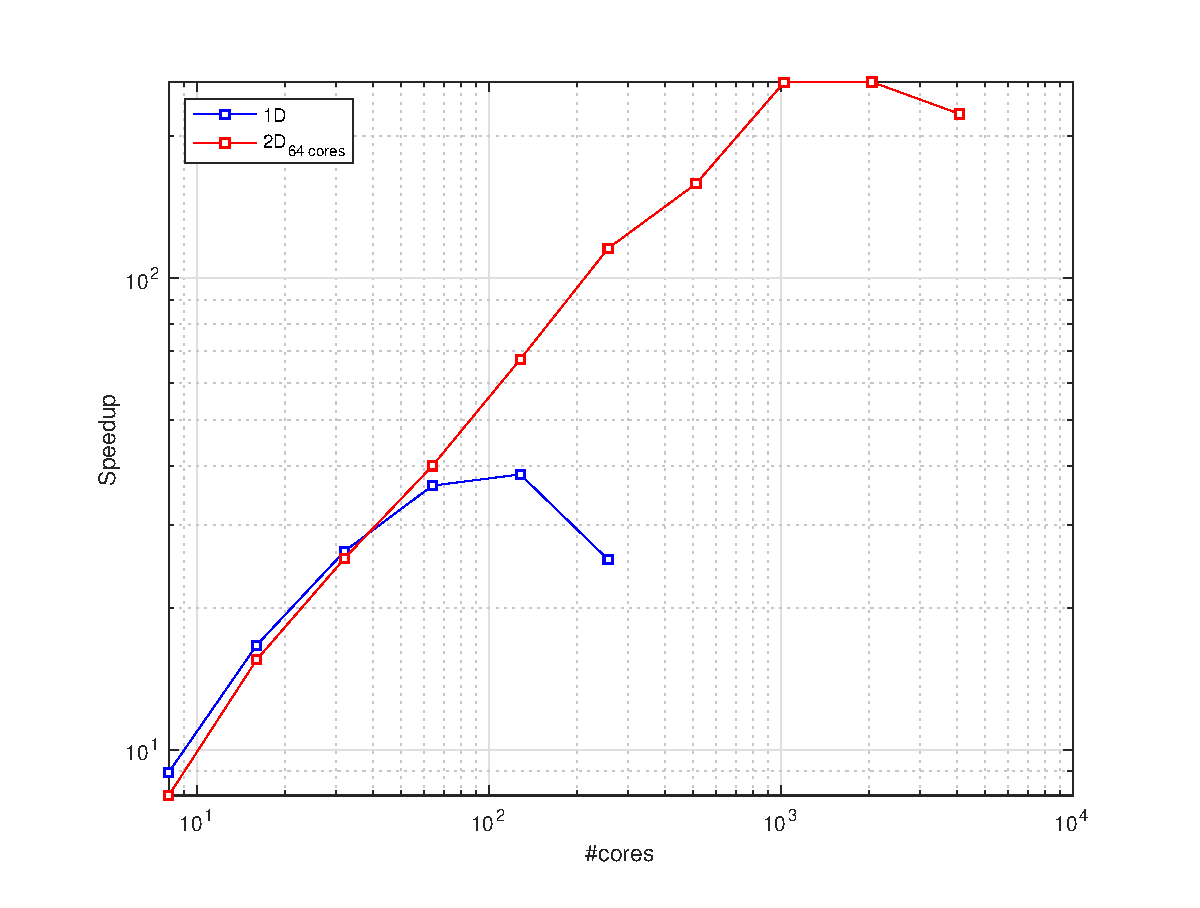
\includegraphics[scale=0.6]{grafici/5122}
\caption{Speedup performance factor of $512^3$ simulation}
\label{5122}
\end{center}
\end{figure}

As we can see from figure~\ref{5122}, the speedup factor of the 2D decomposed algorithm increase approximately linearly until $256$ cores. The raise in performance continue at lower factor until $1024$ cores are reached, where nearly stops before start descending once passed $2048$ cores.
The inverse behavior is shown in figure~\ref{5121}, where the simulation time is plotted against the number of cores.\\
In figure~\ref{5121} is also reported the theoretical scaling limit. Comparing this line, in dashed green, with our results let us conclude that our scaling, although linear for the majority of the time, is sub-optimal. 
The same reasoning is valid also for the slab decomposed algorithm, although in a smaller region of cores number.
It is interesting to denote the advantageous behavior of such algorithm until $64$ cores, where both performances are still slightly different in terms of speedup factor. 
\par
By looking at the values in table~\ref{512data} of page~\pageref{512data} and the depicted counter part, in figures~\ref{5121} and \ref{5122}, it is possible to denote that between $8$ and $16$ cores the loss are really small. This lead us to expect a perfect theoretical linear behavior from $1$ to $16$ cores. Keeping this in mind, we feel confident and seems reasonable to consider a speedup factor of $8$ for the $8$ cores simulation, possibly doing an error below the unit. \\
\par
We refer to figure~\ref{5123} to have an idea of the efficiency of the algorithm. The figure shows that the efficiency remains above $80\%$ until $32$ cores are used. However, once passed such limit, the behavior is linear and smoother with respect to the ones shown in figure~\ref{644} of page~\pageref{644}.

\begin{figure}
\begin{center}
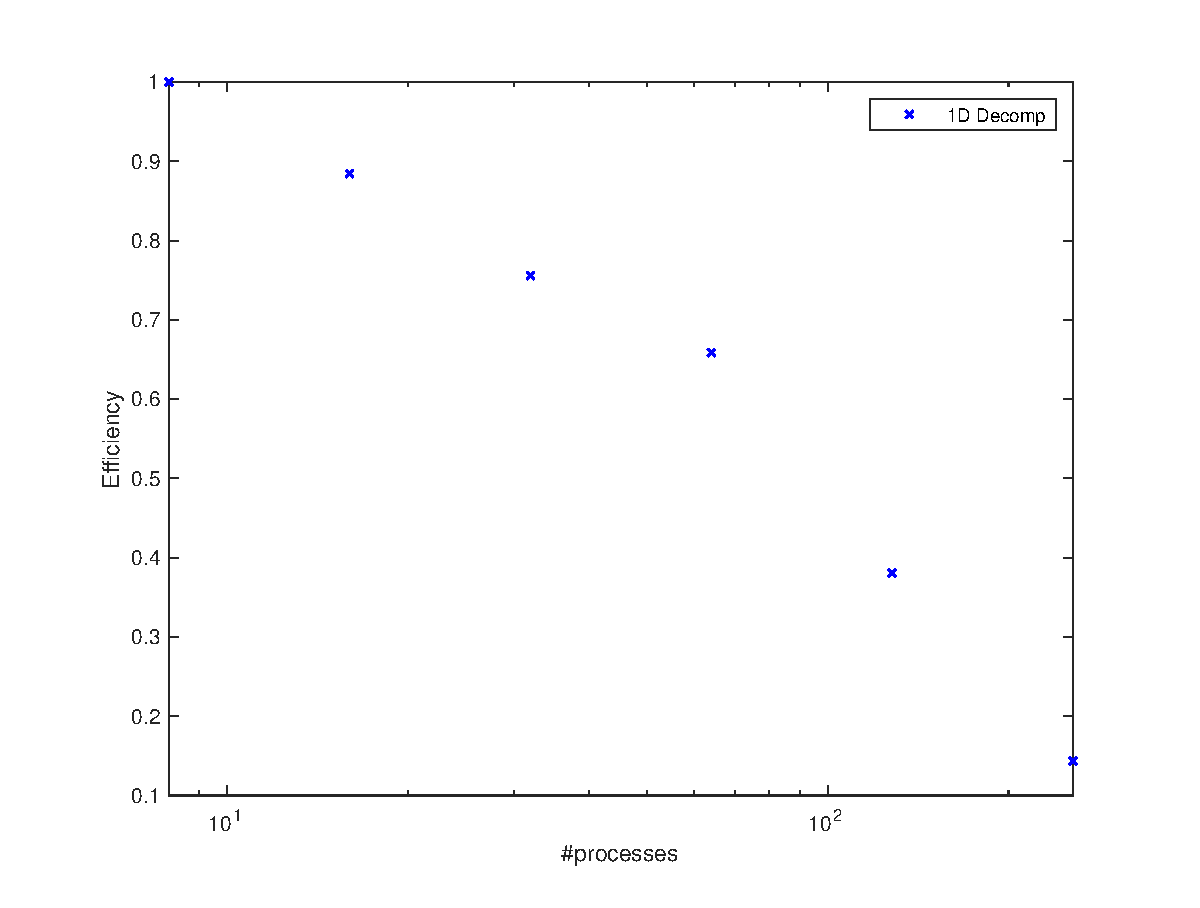
\includegraphics[scale=0.6]{grafici/5123}
\caption{Efficiency factor of $512^3$ simulation}
\label{5123}
\end{center}
\end{figure}


\begin{table}[h]
\caption{Data from $512^{3}$ simulation, if present first row indicates 1D decomposition}
\begin{center}
\begin{tabular}{c c c c}
\toprule
\textbf{\#cores} & \textbf{Time [s]} & \textbf{Speedup} & \textbf{Efficiency [\%]} \\
\midrule
\multirow{2}{*}{8} & 1750 & 8.96 & 112 \\
& 1960 & 1 & 100 \\
\hline
\multirow{2}{*}{16} & 941.5 & 16.65 & 104 \\
& 1011 & 15.51 & 97 \\
\hline
\multirow{2}{*}{32} & 595.3 & 26.35 & 82 \\
& 616.2 & 25.45 & 80 \\
\hline
\multirow{2}{*}{64} & 432.1 & 36.3 & 57 \\
& 392.3 & 39.97 & 62 \\
\hline
\multirow{2}{*}{128} & 409.2 & 38.34 & 30 \\
& 233.2 & 67.22 & 53 \\
\hline
\multirow{2}{*}{256} & 620.1 & 25.29 & 10 \\
& 135.7 & 115.5 & 45 \\
\hline
512 & 99 & 158.4 & 31 \\
1024 & 60.4 & 259.6 & 25 \\

\bottomrule
\end{tabular}
\end{center}
\label{512data}
\end{table}%